% Options for packages loaded elsewhere
\PassOptionsToPackage{unicode}{hyperref}
\PassOptionsToPackage{hyphens}{url}
\PassOptionsToPackage{dvipsnames,svgnames,x11names}{xcolor}
%
\documentclass[
  letterpaper,
  DIV=11,
  numbers=noendperiod]{scrartcl}

\usepackage{amsmath,amssymb}
\usepackage{iftex}
\ifPDFTeX
  \usepackage[T1]{fontenc}
  \usepackage[utf8]{inputenc}
  \usepackage{textcomp} % provide euro and other symbols
\else % if luatex or xetex
  \usepackage{unicode-math}
  \defaultfontfeatures{Scale=MatchLowercase}
  \defaultfontfeatures[\rmfamily]{Ligatures=TeX,Scale=1}
\fi
\usepackage{lmodern}
\ifPDFTeX\else  
    % xetex/luatex font selection
\fi
% Use upquote if available, for straight quotes in verbatim environments
\IfFileExists{upquote.sty}{\usepackage{upquote}}{}
\IfFileExists{microtype.sty}{% use microtype if available
  \usepackage[]{microtype}
  \UseMicrotypeSet[protrusion]{basicmath} % disable protrusion for tt fonts
}{}
\makeatletter
\@ifundefined{KOMAClassName}{% if non-KOMA class
  \IfFileExists{parskip.sty}{%
    \usepackage{parskip}
  }{% else
    \setlength{\parindent}{0pt}
    \setlength{\parskip}{6pt plus 2pt minus 1pt}}
}{% if KOMA class
  \KOMAoptions{parskip=half}}
\makeatother
\usepackage{xcolor}
\setlength{\emergencystretch}{3em} % prevent overfull lines
\setcounter{secnumdepth}{5}
% Make \paragraph and \subparagraph free-standing
\ifx\paragraph\undefined\else
  \let\oldparagraph\paragraph
  \renewcommand{\paragraph}[1]{\oldparagraph{#1}\mbox{}}
\fi
\ifx\subparagraph\undefined\else
  \let\oldsubparagraph\subparagraph
  \renewcommand{\subparagraph}[1]{\oldsubparagraph{#1}\mbox{}}
\fi


\providecommand{\tightlist}{%
  \setlength{\itemsep}{0pt}\setlength{\parskip}{0pt}}\usepackage{longtable,booktabs,array}
\usepackage{calc} % for calculating minipage widths
% Correct order of tables after \paragraph or \subparagraph
\usepackage{etoolbox}
\makeatletter
\patchcmd\longtable{\par}{\if@noskipsec\mbox{}\fi\par}{}{}
\makeatother
% Allow footnotes in longtable head/foot
\IfFileExists{footnotehyper.sty}{\usepackage{footnotehyper}}{\usepackage{footnote}}
\makesavenoteenv{longtable}
\usepackage{graphicx}
\makeatletter
\def\maxwidth{\ifdim\Gin@nat@width>\linewidth\linewidth\else\Gin@nat@width\fi}
\def\maxheight{\ifdim\Gin@nat@height>\textheight\textheight\else\Gin@nat@height\fi}
\makeatother
% Scale images if necessary, so that they will not overflow the page
% margins by default, and it is still possible to overwrite the defaults
% using explicit options in \includegraphics[width, height, ...]{}
\setkeys{Gin}{width=\maxwidth,height=\maxheight,keepaspectratio}
% Set default figure placement to htbp
\makeatletter
\def\fps@figure{htbp}
\makeatother
% definitions for citeproc citations
\NewDocumentCommand\citeproctext{}{}
\NewDocumentCommand\citeproc{mm}{%
  \begingroup\def\citeproctext{#2}\cite{#1}\endgroup}
\makeatletter
 % allow citations to break across lines
 \let\@cite@ofmt\@firstofone
 % avoid brackets around text for \cite:
 \def\@biblabel#1{}
 \def\@cite#1#2{{#1\if@tempswa , #2\fi}}
\makeatother
\newlength{\cslhangindent}
\setlength{\cslhangindent}{1.5em}
\newlength{\csllabelwidth}
\setlength{\csllabelwidth}{3em}
\newenvironment{CSLReferences}[2] % #1 hanging-indent, #2 entry-spacing
 {\begin{list}{}{%
  \setlength{\itemindent}{0pt}
  \setlength{\leftmargin}{0pt}
  \setlength{\parsep}{0pt}
  % turn on hanging indent if param 1 is 1
  \ifodd #1
   \setlength{\leftmargin}{\cslhangindent}
   \setlength{\itemindent}{-1\cslhangindent}
  \fi
  % set entry spacing
  \setlength{\itemsep}{#2\baselineskip}}}
 {\end{list}}
\usepackage{calc}
\newcommand{\CSLBlock}[1]{\hfill\break\parbox[t]{\linewidth}{\strut\ignorespaces#1\strut}}
\newcommand{\CSLLeftMargin}[1]{\parbox[t]{\csllabelwidth}{\strut#1\strut}}
\newcommand{\CSLRightInline}[1]{\parbox[t]{\linewidth - \csllabelwidth}{\strut#1\strut}}
\newcommand{\CSLIndent}[1]{\hspace{\cslhangindent}#1}

\usepackage{booktabs}
\usepackage{longtable}
\usepackage{array}
\usepackage{multirow}
\usepackage{wrapfig}
\usepackage{float}
\usepackage{colortbl}
\usepackage{pdflscape}
\usepackage{tabu}
\usepackage{threeparttable}
\usepackage{threeparttablex}
\usepackage[normalem]{ulem}
\usepackage{makecell}
\usepackage{xcolor}
\KOMAoption{captions}{tableheading}
\makeatletter
\@ifpackageloaded{caption}{}{\usepackage{caption}}
\AtBeginDocument{%
\ifdefined\contentsname
  \renewcommand*\contentsname{Table of contents}
\else
  \newcommand\contentsname{Table of contents}
\fi
\ifdefined\listfigurename
  \renewcommand*\listfigurename{List of Figures}
\else
  \newcommand\listfigurename{List of Figures}
\fi
\ifdefined\listtablename
  \renewcommand*\listtablename{List of Tables}
\else
  \newcommand\listtablename{List of Tables}
\fi
\ifdefined\figurename
  \renewcommand*\figurename{Figure}
\else
  \newcommand\figurename{Figure}
\fi
\ifdefined\tablename
  \renewcommand*\tablename{Table}
\else
  \newcommand\tablename{Table}
\fi
}
\@ifpackageloaded{float}{}{\usepackage{float}}
\floatstyle{ruled}
\@ifundefined{c@chapter}{\newfloat{codelisting}{h}{lop}}{\newfloat{codelisting}{h}{lop}[chapter]}
\floatname{codelisting}{Listing}
\newcommand*\listoflistings{\listof{codelisting}{List of Listings}}
\makeatother
\makeatletter
\makeatother
\makeatletter
\@ifpackageloaded{caption}{}{\usepackage{caption}}
\@ifpackageloaded{subcaption}{}{\usepackage{subcaption}}
\makeatother
\ifLuaTeX
  \usepackage{selnolig}  % disable illegal ligatures
\fi
\usepackage{bookmark}

\IfFileExists{xurl.sty}{\usepackage{xurl}}{} % add URL line breaks if available
\urlstyle{same} % disable monospaced font for URLs
\hypersetup{
  pdftitle={How did local health infrastructure and socio-political factors within different states and counties in the United States affect the disparities in COVID-19 outcomes, and what lessons can be learned for more targeted public health preparedness and response strategies in future pandemics?},
  pdfauthor={Adrian Ly; Sakhil Goel; Hannah Yu},
  colorlinks=true,
  linkcolor={blue},
  filecolor={Maroon},
  citecolor={Blue},
  urlcolor={Blue},
  pdfcreator={LaTeX via pandoc}}

\title{How did local health infrastructure and socio-political factors
within different states and counties in the United States affect the
disparities in COVID-19 outcomes, and what lessons can be learned for
more targeted public health preparedness and response strategies in
future pandemics?\thanks{Code and data are available at:
https://github.com/hannahyu07/US-Covid-Analysis.git}}
\author{Adrian Ly \and Sakhil Goel \and Hannah Yu}
\date{February 12, 2024}

\begin{document}
\maketitle
\begin{abstract}
First sentence. Second sentence. Third sentence. Fourth sentence.
\end{abstract}

\renewcommand*\contentsname{Table of contents}
{
\hypersetup{linkcolor=}
\setcounter{tocdepth}{3}
\tableofcontents
}
\section{Introduction}\label{introduction}

\emph{This reproduction was performed after a replication on the Social
Science Reproduction platform:
}\textbf{\emph{\href{https://www.socialsciencereproduction.org/reproductions/c35e8e98-762d-4c00-a1a3-544ed0b2008d/index}{link
here}}}

\emph{The introduction is self-contained and tells a reader everything
they need to know including: 1) broader context to motivate; 2) some
detail about what the paper is about; 3) a clear gap that needs to be
filled; 4) what was done; 5) what was found; 6) why it is important; 7)
the structure of the paper. A reader should be able to read only the
introduction and know what was done, why, and what was found. Likely 3
or 4 paragraphs, or 10 per cent of total. The estimand is clearly stated
in the introduction.}

\section{Data}\label{sec-data}

Our results are summarized in (\textbf{fig:fig-GHS?}).

\subsection{Source}\label{source}

The datasets utilized in this paper were mainly obtained from the
\texttt{original\ paper} (Nuzzo and Ledesma 2023). Additionally, to
address the original paper's lack of US Covid statistics and political
party support data, we incorporated information from Jack and Oster
(2023) and Elflein (2023).

Jack and Oster (2023) discusses the long-term impacts of COVID-related
school closures. From this source, we utilized the dataset on voting
shares during the 2020 election by county. Elflein (2023) provides
summaries of COVID-19 death rates in the United States as of March 2023,
organized by state. Analyzing results from both datasets allows us to
explore the relationship between political affiliation and COVID-19
outcomes.Our reproduction aims to fill these gaps and also includes
tables and graphs that were not presented in the original paper to
support our findings.

\subsection{Methodology}\label{methodology}

\texttt{R} (R Core Team 2022) was the language and environment used for
the bulk of this analysis, alongside \texttt{tidyverse} (Wickham et al.
2019), \texttt{sf} (Pebesma 2018), \texttt{readxl} (Wickham and Bryan
2023), \texttt{knitr} (Xie 2014), \texttt{janitor} (Firke 2023),
\texttt{lubridate} (Grolemund and Wickham 2011), \texttt{dplyr} (Wickham
et al. 2023), \texttt{data.table} (Barrett et al. 2024),
\texttt{RColorBrewer} (Neuwirth 2022), \texttt{ggpubr} (Kassambara
2023), \texttt{ggplot2} (Wickham 2016), \texttt{here} (Müller 2020),
\texttt{kableExtra} (Zhu 2024), \texttt{webshot} (Chang 2023a),
\texttt{webshot2} (Chang 2023b), \texttt{gt} (Iannone et al. 2024), and
\texttt{scales} (Wickham, Pedersen, and Seidel 2023).

\subsection{Data Measurement}\label{data-measurement}

\emph{A thorough discussion of measurement, relating to the dataset, is
provided in the data section.}

\subsection{Data cleaning}\label{data-cleaning}

\begin{figure}

\centering{

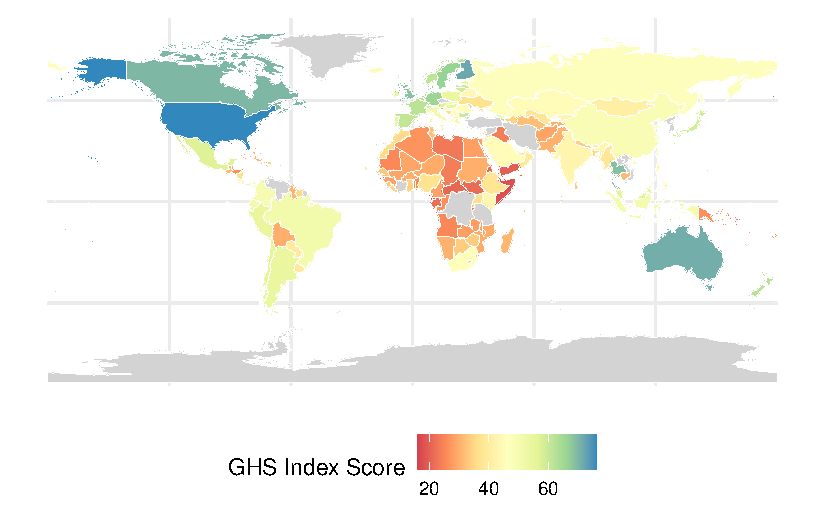
\includegraphics{paper_files/figure-pdf/fig-GHS-1.pdf}

}

\caption{\label{fig-GHS}Global Health Security Index Scores by Country}

\end{figure}%

\section{Results}\label{results}

Our results are summarized in the following figures. \textbf{?@fig-ELE}
illustrates the trend of life expectancy at birth across different
racial groups over time. Table~\ref{tbl-life_exp} provides a more
detailed breakdown of the life expectancy before and during COVID
for\ldots{} Unfortunately, due to the unavailability of data over time
for Asians and American Indian and Alaska Native communities, they have
been excluded from the time series graph.

An intriguing observation is the consistently higher life expectancy
among Hispanic individuals compared to other groups, even amidst the
challenges posed by COVID-19. On the other hand, Black individuals l
have consistently exhibited lower life expectancy, which further
declined notably in 2021, reaching just over 70.8 years old. The life
expectancy trends of white people and all other races and origins remain
close together throughout the 14 year time period, with minimum
variance. Specifically, the life expectancy for White individuals
decreased from 78.8 to 76.4 years old from pre-pandemic levels in 2019
to 2021, while for Hispanic individuals, it dropped by 4.2 years, and
for Black individuals, it declined by 4 years during the same period.

\begin{table}

\caption{\label{tbl-life\_exp}Life Expectancy by Race (2019-2021)}

\centering{

}

\end{table}%

\begin{figure}

\centering{

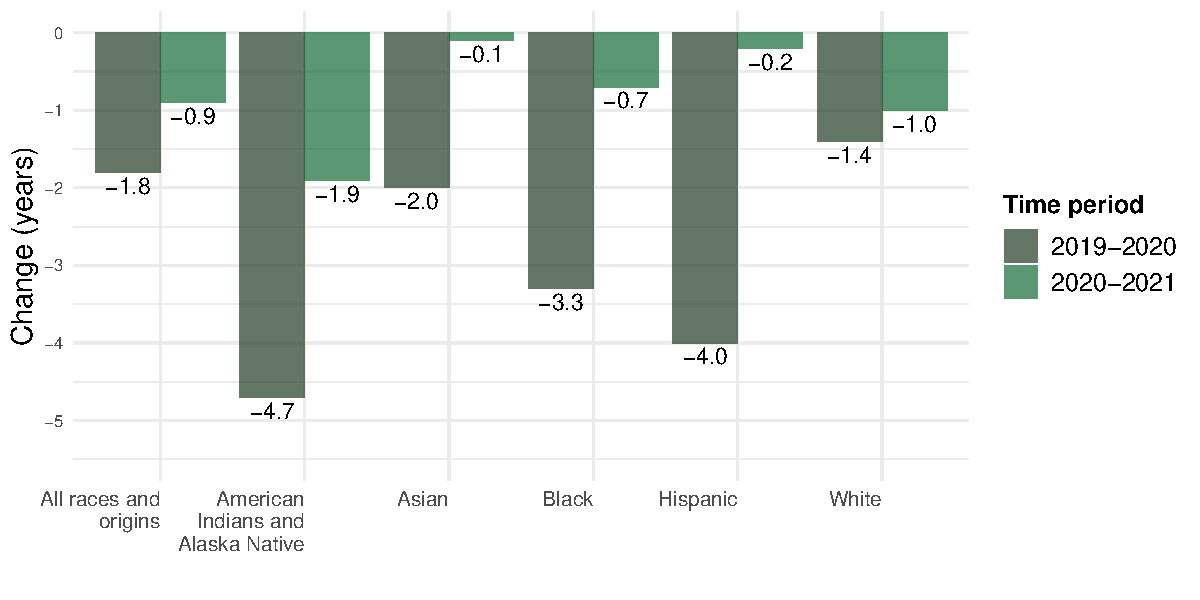
\includegraphics{paper_files/figure-pdf/fig-CLE-1.pdf}

}

\caption{\label{fig-CLE}Change in Life Expectancy at Birth from the
Previous Year}

\end{figure}%

Figure~\ref{fig-CLE} serves as a valuable addition to our previous
analysis with the inclusion of Asians and American Indians and Alaska
Natives during the critical period from 2019 to 2021. With these
additional ethnic categories, we can discern that American Indians and
Alaska Natives experienced significant impacts from the pandemic, with a
decrease of 4.7 years in the first year and 1.9 years in the second
year, totaling 6.6 years.

With a chart that depicts the change of life expectancy each year by
ethnicity, we are able to better gain a more comprehensive understanding
of the impact of COVID by ethnicity. While the declines in life
expectancy are smaller in magnitude from 2020 to 2021, they are notably
minimal for Asians and Hispanics, with reductions of -0.1 and -0.2 years
respectively. (Insert some sources tmrw)

Numerous sources have indicated a correlation between a state's
political affiliation and its handling of COVID issues (sources to be
inserted tomorrow). To testify the claim, we collected the voting data
for each of the 50 states for the 2020 presidential election. We then
selected the ten states with the highest proportions of Republican
votes.These voting patterns are visualized in Figure
Figure~\ref{fig-Vote}, where red symbols represent Republican votes and
blue symbols represent Democratic votes. Among the top ten states,
Tennessee recorded the highest total number of votes, while Wyoming
boasted the highest proportion of Republican votes.

\begin{figure}

\centering{

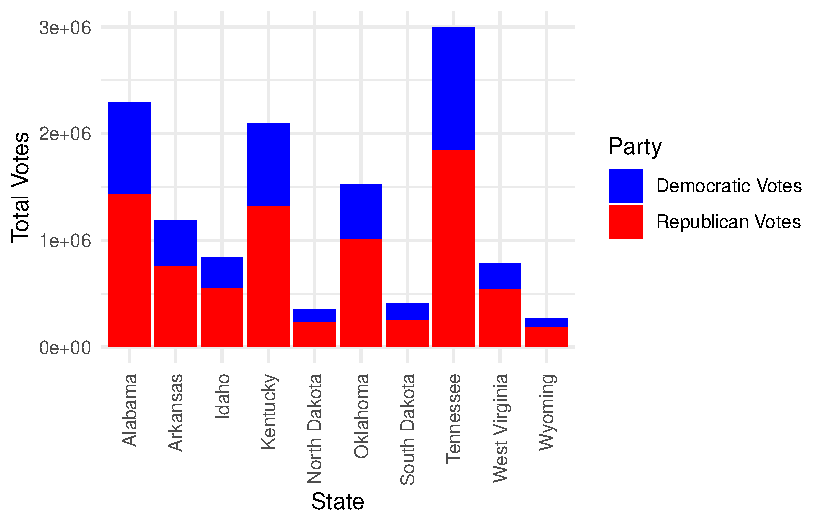
\includegraphics{paper_files/figure-pdf/fig-Vote-1.pdf}

}

\caption{\label{fig-Vote}Total Number of Votes in Top 10 States with
Highest Proportion of Republican Votes}

\end{figure}%

Given the variation in population sizes among states, direct comparisons
of COVID case numbers are inherently flawed. As an alternative, we
employed death rates per 100,000 people as a metric for evaluating each
state's COVID preparedness and situation. We then produced
Table~\ref{tbl-deaths} that ranks the top ten states with the highest
death rates from COVID per 100,000 people to examine the potential
correlation between party preferences and COVID related deaths. Notably,
We found that six of the ten top Republican states made a reappearance
in the top death rates table; these states are Oklahoma, West Virginia,
Arkansas, Alabama, Tennessee, and Kentucky. (Insert quotes about
republican party and covid tmrw)

\begin{table}

\caption{\label{tbl-deaths}Top 10 States with Highest Death Rates from
COVID-19 (per 100,000 people)}

\centering{

}

\end{table}%

Following from our previous analysis regarding individuals' political
affiliations, we have developed Figure
Figure~\ref{fig-deaths_rates_votes}, which encompasses all 50 states of
the US along with their political leanings based on which party garnered
the majority votes. This information is juxtaposed against their
respective COVID death rates.

While we cannot make any definitive assertions about stark differences,
we do observe that the Republican-leaning states are slightly more
clustered around higher death rates ranging from 350 to 450 deaths,
while the Democratic-leaning states appear to be more evenly
distributed, and notably one Democratic-leaning state has the lowest
death rate.An intriguing observation is that although many
Republican-leaning states demonstrate higher COVID death rates, it is
noteworthy that Arizona, typically considered a Democratic-leaning
state, records the highest death rate among all states.

(may add more)

\begin{figure}

\centering{

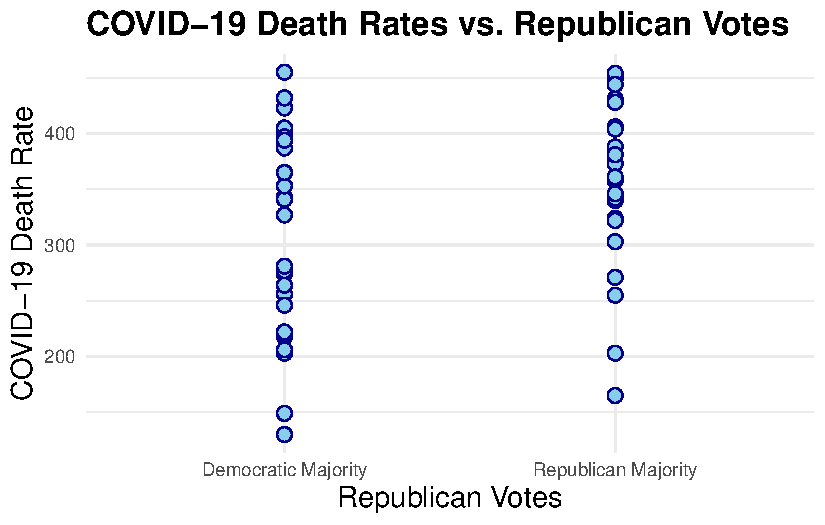
\includegraphics{paper_files/figure-pdf/fig-deaths_rates_votes-1.pdf}

}

\caption{\label{fig-deaths\_rates\_votes}COVID-19 Death Rates
vs.~Republican Votes}

\end{figure}%

\newpage

\section{Discussion}\label{discussion}

This begs the question as to why we are seeing these results. There
isn't exactly a single answer to this question, however we can certainly
point out some considerable factors to this result.

\subsection{Influence of political polarization on adherence to health
guidelines.}\label{influence-of-political-polarization-on-adherence-to-health-guidelines.}

Political polarization has significantly impacted the adherence to
health guidelines during the COVID-19 pandemic. The divergence in
political ideologies has translated into differing attitudes towards
health directives, including mask mandates, social distancing, and
vaccination uptake.

Various studies and our own results have shown that areas with higher
support for one political party exhibited distinct behaviors and
compliance levels with health recommendations, which directly correlated
with COVID-19 case rates and mortality. An news article from
\texttt{ABC\ News} (Diab and Kumar 2023) shows that the top states with
the highest COVID-19 deaths are Arizona, and Washington with 581 deaths
and 526 deaths respectively per 100,000 people. According to 2020
presidential voting data published by \texttt{CNN}, we have both states
having the electoral vote of democrat with Washington wining by 58\%
(\emph{2020 Election Results by State, Washington} 2020) and Arizona
winning by 49.4\% (\emph{2020 Election Results by State, Arizona} 2020).
Another news article by \texttt{ContagionLive} (Parkinson 2023) also
makes the claim of both Arizona and Washington having the highest
COVID-19 mortality. This polarization has not only influenced individual
behavior but also shaped state and local health policies, further
entrenching the disparities in health outcomes.

The adherence to health guidelines are evident in the varied health
outcomes observed across the United States. Regions with lower
compliance to health directives, often influenced by political leanings,
have experienced higher rates of COVID-19 transmission,
hospitalizations, and deaths. The disparities in vaccine uptake, driven
by political affiliations, have further exacerbated these outcomes,
leaving certain communities more vulnerable to the virus and its
variants. In order to mitigate the influence of political polarization
on public health, it is imperative to depoliticize health guidelines and
focus on evidence-based approaches to disease prevention and control.
Building trust in health institutions and promoting bipartisan support
for public health measures are essential steps towards achieving higher
compliance and better health outcomes. Engaging trusted community
leaders and utilizing targeted communication strategies can also help
bridge the divide and encourage adherence to health guidelines.

\subsection{Impact of government transparency and consistent
communication on public
trust.}\label{impact-of-government-transparency-and-consistent-communication-on-public-trust.}

The politicization of health guidelines and mixed messages from
political and health leaders during the COVID-19 pandemic have
significantly undermined the effectiveness of public health messaging,
leading to confusion, skepticism, and eroded trust among the public.
Initially, inconsistencies in recommendations, such as on mask usage,
challenged the principle of clear, consistent, and science-based
communication essential for an effective public health response.
Moreover, the transparency of government actions and decision-making
processes is crucial in building and maintaining public trust,
especially during health crises. The level of public trust was greatly
affected by the openness and accuracy with which governments, at all
levels, communicated about the evolving situation, the reasoning behind
guidelines, and the measures taken to combat the virus, emphasizing the
importance of transparent reporting of data related to case counts,
hospitalizations, vaccine distribution, and side effects. Furthermore,
consistent communication from public health officials and government
leaders is key to ensuring adherence to health guidelines, where
inconsistencies, such as changes in mask-wearing guidelines without
clear explanations, have led to public confusion. The direct correlation
between government transparency, consistent communication, and public
behavior is self-evident, with populations receiving clear and
transparent information being more likely to adhere to guidelines,
participate in testing and tracing efforts, and accept vaccination.
Drawing lessons from the pandemic, strategies for improving government
transparency and communication in future health emergencies should
include establishing centralized information hubs, ensuring regular and
predictable communication from health authorities, engaging community
leaders in information dissemination, and harnessing digital platforms
and social media to amplify public health messages, thus reinforcing
public trust and compliance.

\subsection{Role of social vulnerabilities and healthcare access
disparities in pandemic
impact.}\label{role-of-social-vulnerabilities-and-healthcare-access-disparities-in-pandemic-impact.}

\subsection{Strategies for improving real-time data collection and
sharing for public health
decisions.}\label{strategies-for-improving-real-time-data-collection-and-sharing-for-public-health-decisions.}

To address the fragmentation in data collection and sharing witnessed
during the pandemic, it's crucial to establish integrated data platforms
that enable seamless health data exchange among various health agencies
and stakeholders, utilizing cloud computing and APIs for real-time
accessibility and usability. Equally important is enhancing data
standardization and interoperability through universal standards like
FHIR (Fast Healthcare Interoperability Resources) to facilitate
efficient data sharing. Investing in digital surveillance systems, which
employ AI and machine learning to sift through diverse data sources for
early outbreak detection, is essential for rapid response to health
threats. Furthermore, fostering public-private partnerships can harness
the agility of the private sector and the public health expertise of
governmental agencies to enhance data analytics capabilities. Ensuring
the privacy and security of health data through robust governance
frameworks and advanced encryption is paramount to maintaining public
trust. Engaging communities in these initiatives ensures their relevance
and fosters trust, while building global data sharing networks
encourages international collaboration, crucial for a concerted response
to pandemics. Collectively, these strategies are fundamental to
bolstering public health decision-making and preparedness, making our
health systems more resilient against the challenges posed by emerging
infectious diseases.

\subsection{Weaknesses and next steps}\label{weaknesses-and-next-steps}

Weaknesses and next steps should also be included.

\newpage

\section*{References}\label{references}
\addcontentsline{toc}{section}{References}

\phantomsection\label{refs}
\begin{CSLReferences}{1}{0}
\bibitem[\citeproctext]{ref-citesource3}
\emph{2020 Election Results by State, Arizona}. 2020. CNN.
\url{https://www.cnn.com/election/2020/results/state/arizona}.

\bibitem[\citeproctext]{ref-citesource2}
\emph{2020 Election Results by State, Washington}. 2020. CNN.
\url{https://www.cnn.com/election/2020/results/state/washington}.

\bibitem[\citeproctext]{ref-citeDataTable}
Barrett, Tyson, Matt Dowle, Arun Srinivasan, Jan Gorecki, Michael
Chirico, and Toby Hocking. 2024. \emph{Data.table: Extension of
`Data.frame`}. \url{https://CRAN.R-project.org/package=data.table}.

\bibitem[\citeproctext]{ref-citewebshot}
Chang, Winston. 2023a. \emph{Webshot: Take Screenshots of Web Pages}.
\url{https://CRAN.R-project.org/package=webshot}.

\bibitem[\citeproctext]{ref-citewebshot2}
---------. 2023b. \emph{Webshot2: Take Screenshots of Web Pages}.
\url{https://CRAN.R-project.org/package=webshot2}.

\bibitem[\citeproctext]{ref-citesource1}
Diab, Dr. Alaa, and Dr. Keerthana Kumar. 2023. \emph{COVID-19 Death
Rates Varied Dramatically Across US, Major Analysis Finds}. ABC News.
\url{https://abcnews.go.com/Health/covid-19-death-rates-varied-dramatically-us-major/story?id=98055024}.

\bibitem[\citeproctext]{ref-citedata2}
Elflein, John. 2023. {``U.s. COVID-19 Death Rate by State.''}
\emph{Statista}.
\url{https://www.statista.com/statistics/1109011/coronavirus-covid19-death-rates-us-by-state/}.

\bibitem[\citeproctext]{ref-citeJanitor}
Firke, Sam. 2023. \emph{Janitor: Simple Tools for Examining and Cleaning
Dirty Data}. \url{https://CRAN.R-project.org/package=janitor}.

\bibitem[\citeproctext]{ref-citeLubridate}
Grolemund, Garrett, and Hadley Wickham. 2011. {``Dates and Times Made
Easy with {lubridate}.''} \emph{Journal of Statistical Software} 40 (3):
1--25. \url{https://www.jstatsoft.org/v40/i03/}.

\bibitem[\citeproctext]{ref-citeGT}
Iannone, Richard, Joe Cheng, Barret Schloerke, Ellis Hughes, Alexandra
Lauer, and JooYoung Seo. 2024. \emph{Gt: Easily Create
Presentation-Ready Display Tables}.
\url{https://CRAN.R-project.org/package=gt}.

\bibitem[\citeproctext]{ref-citedata1}
Jack, Rebecca, and Emily Oster. 2023. {``COVID-19, School Closures, and
Outcomes.''} \emph{Journal of Economic Perspectives} 37 (4): 51--70.
https://doi.org/\url{https://doi.org/10.1257/jep.37.4.51}.

\bibitem[\citeproctext]{ref-citeggpubr}
Kassambara, Alboukadel. 2023. \emph{Ggpubr: 'Ggplot2' Based Publication
Ready Plots}. \url{https://CRAN.R-project.org/package=ggpubr}.

\bibitem[\citeproctext]{ref-citeHere}
Müller, Kirill. 2020. \emph{Here: A Simpler Way to Find Your Files}.
\url{https://CRAN.R-project.org/package=here}.

\bibitem[\citeproctext]{ref-citeRColorBrewer}
Neuwirth, Erich. 2022. \emph{RColorBrewer: ColorBrewer Palettes}.
\url{https://CRAN.R-project.org/package=RColorBrewer}.

\bibitem[\citeproctext]{ref-citearticle}
Nuzzo, Jennifer B., and Jorge R. Ledesma. 2023. \emph{Why Did the Best
Prepared Country in the World Fare so Poorly During COVID?}
\url{https://www.aeaweb.org/articles?id=10.1257/jep.37.4.3}.

\bibitem[\citeproctext]{ref-citesource4}
Parkinson, John. 2023. \emph{Which States Saw Greatest COVID-19
Mortality?} ContagionLive.
\url{https://www.contagionlive.com/view/which-states-saw-greatest-covid-19-mortality-}.

\bibitem[\citeproctext]{ref-citeSF}
Pebesma, Edzer. 2018. {``{Simple Features for R: Standardized Support
for Spatial Vector Data}.''} \emph{{The R Journal}} 10 (1): 439--46.
\url{https://doi.org/10.32614/RJ-2018-009}.

\bibitem[\citeproctext]{ref-citeR}
R Core Team. 2022. \emph{R: A Language and Environment for Statistical
Computing}. Vienna, Austria: R Foundation for Statistical Computing.
\url{https://www.R-project.org/}.

\bibitem[\citeproctext]{ref-citeggplot}
Wickham, Hadley. 2016. \emph{Ggplot2: Elegant Graphics for Data
Analysis}. Springer-Verlag New York.
\url{https://ggplot2.tidyverse.org}.

\bibitem[\citeproctext]{ref-citeTidyVerse}
Wickham, Hadley, Mara Averick, Jennifer Bryan, Winston Chang, Lucy
D'Agostino McGowan, Romain François, Garrett Grolemund, et al. 2019.
{``Welcome to the {tidyverse}.''} \emph{Journal of Open Source Software}
4 (43): 1686. \url{https://doi.org/10.21105/joss.01686}.

\bibitem[\citeproctext]{ref-citeReadXL}
Wickham, Hadley, and Jennifer Bryan. 2023. \emph{Readxl: Read Excel
Files}. \url{https://CRAN.R-project.org/package=readxl}.

\bibitem[\citeproctext]{ref-citeDplyr}
Wickham, Hadley, Romain François, Lionel Henry, Kirill Müller, and Davis
Vaughan. 2023. \emph{Dplyr: A Grammar of Data Manipulation}.
\url{https://CRAN.R-project.org/package=dplyr}.

\bibitem[\citeproctext]{ref-citeScales}
Wickham, Hadley, Thomas Lin Pedersen, and Dana Seidel. 2023.
\emph{Scales: Scale Functions for Visualization}.
\url{https://CRAN.R-project.org/package=scales}.

\bibitem[\citeproctext]{ref-citeKnitR}
Xie, Yihui. 2014. {``Knitr: A Comprehensive Tool for Reproducible
Research in {R}.''} In \emph{Implementing Reproducible Computational
Research}, edited by Victoria Stodden, Friedrich Leisch, and Roger D.
Peng. Chapman; Hall/CRC.

\bibitem[\citeproctext]{ref-citeKableExtra}
Zhu, Hao. 2024. \emph{kableExtra: Construct Complex Table with 'Kable'
and Pipe Syntax}. \url{https://CRAN.R-project.org/package=kableExtra}.

\end{CSLReferences}



\end{document}
